\documentclass[11pt]{article}
\usepackage{graphicx}
\usepackage{amssymb}
\usepackage{epstopdf}
\usepackage{subfigure}

\usepackage{ucs}
\usepackage[utf8x]{inputenc}
\usepackage[T1]{fontenc}
\newcommand{\textGamma}{\ensuremath{\Gamma}}
\newcommand{\textDelta}{\ensuremath{\Delta}}
\newcommand{\textalpha}{\ensuremath{\alpha}}
\newcommand{\textbeta}{\ensuremath{\beta}}
\newcommand{\textlambda}{\ensuremath{\lambda}}
\DeclareUnicodeCharacter {8614}{\ensuremath{|->}}
\DeclareUnicodeCharacter {8870}{\ensuremath{|-}}
\DeclareUnicodeCharacter {8871}{\ensuremath{|=}}
\DeclareUnicodeCharacter {9665}{\ensuremath{\triangleleft}}

\hoffset = 0mm
\voffset = 0mm
\textwidth = 165mm
\textheight = 229mm
\oddsidemargin = 0.0 in
\evensidemargin = 0.0 in
\topmargin = 0.0 in
\headheight = 0.0 in
\headsep = 0.0 in
\parskip = 3pt
\parindent = 0.0in

\makeatletter
\renewcommand{\@makefntext}[1]{\setlength{\parindent}{0pt}%
\begin{list}{}{\setlength{\labelwidth}{1em}%
  \setlength{\leftmargin}{\labelwidth}%
  \setlength{\labelsep}{3pt}\setlength{\itemsep}{0pt}%
  \setlength{\parsep}{0pt}\setlength{\topsep}{0pt}%
  \footnotesize}\item[\hfill\@makefnmark]#1%
\end{list}}
\makeatother

\usepackage{graphicx}
\usepackage{amssymb, amsmath}
\usepackage{proof} 
\usepackage{stmaryrd}
\input{mapsto}

\usepackage[ligature,reserved]{semantic}

\reservestyle{\word}{\operatorname}

\reservestyle{\bracket}{\mathsf}
\bracket{if[if\;],then[\;then\;],nlthen[then\;],else[\;else\;],nlelse[else\;],elsf[\;elsf\;],nlelsf[elsf\;],fi[\;fi],nlfi[fi],
	while[while\;],do[\;do\;],nldo[do\;],od[\;od],nlod[od],
	untildo[do\;],until[\;until\;],nluntil[until\;]}
\bracket{let[let\;],letand[\;and\;],local[local\;],in[\;in\;],ni[\;ni]}
\bracket{with[with\;],when[\;when\;],}
\bracket{resource[resource\;]}

\reservestyle{\predicate}{\mathrm}
\predicate{P,V}

\reservestyle{\instruction}{\mathrm}
\instruction{skip}

\reservestyle{\constructor}{\mathsf}

\reservestyle{\var}{\mathit}

\reservestyle{\const}{\mathrm}
\const{nil,true,false}

\reservestyle{\bconst}{\mathbf}
\bconst{emp,emph[emp_{h}],emps[emp_{s}]}

\DeclareMathOperator{\new}{new}
\DeclareMathOperator{\dispose}{dispose}
\DeclareMathOperator{\notop}{not}
\DeclareMathOperator{\invop}{bitinv}

% mathligs must be arranged in reverse prefix order
\mathlig{--*}{\mathbin{-\!\circledast}}
\mathlig{-*}{\mathbin{-\!\!\star}}
\mathlig{*}{\star}
\mathlig{|->}{\mapsto}
\mathlig{||-}{\Vdash}
\mathlig{|-}{\vdash}
\mathlig{|=}{\vDash}
\mathlig{|*}{\exists}
\mathlig{[|}{\llbracket} % stmaryrd open semantic bracket
\mathlig{|]}{\rrbracket} % stmaryrd close semantic bracket
\mathlig{|}{\lor}
\mathlig{@**}{\forall\circledast} % iterated separating conjunction
\mathlig{@*}{\forall}
\mathlig{@+}{\oplus}
\mathlig{@@@@}{@}
\mathlig{@}{\land}
\mathlig{/->}{\hookrightarrow}
\mathlig{->}{\rightarrow}
\mathlig{=>}{\Rightarrow}
\mathlig{!/->}{\not\hookrightarrow}
\mathlig{!=>}{\not\Rightarrow}
\mathlig{!=}{\neq}
\mathlig{!|-}{\not\vdash}
\mathlig{!||-}{\not\Vdash}
\mathlig{!|=}{\not\,\vDash}
\mathlig{!|*}{\neg\exists}%necessary before !|
\mathlig{!|}{\not\!\lor}
\mathlig{!@*}{\neg\forall}%necessary before !@
\mathlig{!@}{\not\!\!\land}
\mathlig{!}{\neg}
\mathlig{>=}{\geq}
\mathlig{>->}{\rightarrowtail}
\mathlig{~>}{\rightsquigarrow}
\mathlig{~<>}{\leftrightsquigarrow}
\mathlig{~<}{\leftsquigarrow}
\mathlig{<->}{\leftrightarrow}
\mathlig{<=>}{\iff}
\mathlig{<=}{\leq}

\newcommand {\singl}[1]{\langle #1 \rangle}
\newcommand {\mtseq}{\singl{\,}}
%
% To make arrays within math environments
%
\newcommand {\cols}[1][*{50}{l}]{\begin{array}{#1}}
\newcommand {\sloc}{\end{array}}
\newcommand {\defin}{\cols[rcl]}
\newcommand {\nifed}{\sloc}
\newcommand {\BRA}[1][*{50}{l}]{\left(\cols[#1]}
\newcommand {\KET}{\sloc\right)}
\newcommand {\BRACE}[1][*{50}{l}]{\left\{\cols[#1]}
\newcommand {\ECARB}{\sloc\right\}}
\newcommand {\LANG}[1][*{50}{l}]{\left\langle\cols[#1]}
\newcommand {\GNAL}{\sloc\right\rangle}
\newcommand {\FRAME}[1][l]{\text{Framed:}\left\langle\begin{array}{#1}}
\newcommand {\EMARF}{\end{array}\right\rangle}

\mathlig{++}{\mathbin{+\!\,+}}
\mathlig{--}{\mathbin{-\!\,-}}

\newcommand{\assert}[1]{\left\{ #1 \right\}}
\newcommand{\Assert}[1]{\BRACE #1 \ECARB}

\newcommand{\pre}[1]{\assert{#1}\,}
\newcommand{\Pre}[1]{\Assert{#1}\,}
\newcommand{\post}[1]{\,\assert{#1}}
\newcommand{\Post}[1]{\,\Assert{#1}}
\newcommand{\mida}[1]{\,\assert{#1}\,}
\newcommand{\Mida}[1]{\,\Assert{#1}\,}

\newcommand{\eqnlabel}[1]{\label{eqn:#1}}
\newcommand{\eqnref}[1]{(\ref{eqn:#1})}
\newcommand{\figlabel}[1]{\label{fig:#1}}
\newcommand{\figref}[1]{figure \ref{fig:#1}}
\newcommand{\Figref}[1]{Figure \ref{fig:#1}}
\newcommand{\seclabel}[1]{\label{sec:#1}}
\newcommand{\secref}[1]{section \ref{sec:#1}}
\newcommand{\Secref}[1]{Section \ref{sec:#1}}
\newcommand{\tablabel}[1]{\label{tab:#1}}
\newcommand{\tabref}[1]{table \ref{tab:#1}}
\newcommand{\Tabref}[1]{Table \ref{tab:#1}}
\newcommand{\deflabel}[1]{\label{def:#1}}
\newcommand{\defref}[1]{definition \ref{def:#1}}
\newcommand{\Defref}[1]{lemma \ref{def:#1}}
\newcommand{\lemlabel}[1]{\label{lem:#1}}
\newcommand{\lemref}[1]{lemma \ref{lem:#1}}
\newcommand{\Lemref}[1]{Lemma \ref{lem:#1}}

\newenvironment{progindent}{\quad\cols}{\sloc}

\newcommand{\hstrut}[1]{\rule{#1}{0pt}}
\newcommand{\vstrut}[1]{\rule{0pt}{#1}}

\newcommand{\vgap}[1]{\vstrut{#1} \\}

\newcommand{\eqnscale}{0.8}
\newcommand{\reasonscale}{0.8}
\newcommand{\picscale}{0.8}

\newcommand{\seqn}[1]{\begin{equation}\scalebox{\eqnscale}{$#1$}\end{equation}}

\newcommand{\inferR}[3][]{\infer[\scalebox{\reasonscale}{$#1$}]{#2}{#3}}
\newcommand{\eqdef}{\stackrel{\text{\tiny def}}{=}}

 

%\reservestyle{\word}{\operatorname}
\newcommand{\reason}[1]{\scalebox{0.7}{#1}}
\renewcommand{\picscale}{0.6}

\newenvironment{japeish}{\begin{quote}\tt\small}{\end{quote}}
\newcommand{\textj}[1]{{\tt\small{#1}}}

\title{Forward reasoning in Jape}
\author{Richard Bornat \\ School of Computing Science, Middlesex University, UK
}
\begin{document}
\maketitle

\begin{abstract}
\noindent

\end{abstract}

\section{Introduction}

Jape began, back in 1992, as a joint project with Bernard Sufrin to build a proof calculator\footnote{We called it a proof `editor', but it was always in fact a calculator.} with a convenient user interface, covering lots of different kinds of user-defined logics with user-configurable automation of the proof calculation process. We didn't know how hard it would be to hit some of those goals. In the end I converted most of the automation mechanism into support for the convenient user interface.

One strand of work which bore fruit was the support for `box and line' proofs, and this note sets out the design and explains the mechanisms which you can use to do the same thing. It isn't easy to do, and in setting it up I've undermined one of Bernard's original purposes, which was to make Jape easy to configure. Now that I know some of the complexities of supporting proof calculation, I think that perhaps Jape is too general for its own good, and that box and line proofs should be supported by a special natural deduction tool. But I haven't built such a tool, so there follows a description of how to do it in Jape.

\section{Tree and box display}

Jape's first logic encoding was a single-conclusion intuitionistic sequent calculus, with the rules shown in \tabref{SCS}. This is, as Mark Dawson pointed out in the thesis~\cite{Dawsonthesis1990,DawsonGenericlogicenvironment1992} which inspired us in the early days of Jape, an `all-introduction' calculus: at each step a rule reduces either a hypothesis (left-side) or a conclusion (right-side) formula at a tip of a tree of sequents, generating new tips or (with axioms hyp and ⊥⊢) closing the tip. It's then natural to build tree proofs step by step like the partial attempt in \figref{firsttree}, working backwards from the target sequent towards the tips of the final proof tree.

\begin{table}[t]
\footnotesize
\centering
\caption{The rules of the single-conclusion intuitionistic sequent calculus}
\label{tab:SCS}
\vstrut{20pt}
$\infer[\reason{hyp}]
       {\Gamma,A |- A }
       {}$ 
\\
\vstrut{40pt}
$\infer[\reason{⊦∧}]
       {\Gamma  |- A@B }
       {\Gamma  |- A & \Gamma  |- B }$
\qquad\vstrut{30pt}
$\infer[\reason{⊦→}]
       {\Gamma  |- A->B }
       {\Gamma,A |- B }$
\qquad\vstrut{30pt}
$\infer[\reason{⊦∨(L)}]
       {\Gamma  |- A|B }
       {\Gamma  |- A }$
$\infer[\reason{⊦∨(R)}]
       {\Gamma  |- A|B }
       {\Gamma  |- B }$
\\
\qquad\vstrut{30pt}
$\infer[\reason{⊦¬ }]
       {\Gamma |- !A }
       {\Gamma |- A->\bot }$ 
\qquad\vstrut{30pt}
$\infer[\reason{⊦≡}]
       {\Gamma |- A\equiv B }
       {\Gamma |- A->B & \Gamma |- B->A }$
\\
\qquad\vstrut{30pt}
$\infer[\reason{(fresh $m$) ⊦∀}]
       {\Gamma  |- @*x.P(x) }
       {\Gamma  |- P(m) }$
\qquad\vstrut{30pt}
$\infer[\reason{⊦∃}]
       {\Gamma  |-|*x.P(x) }
       {\Gamma  |- P(E) }$
\\
\vstrut{40pt}
$\infer[\reason{∧⊦}]
       {\Gamma,A@B |- C }
       {\Gamma,A,B |- C }$
\qquad\vstrut{30pt}
$\infer[\reason{→⊦}]
       {\Gamma,A->B |- C }
       {\Gamma  |- A & \Gamma,B |- C }$
\qquad\vstrut{30pt}
$\infer[\reason{∨⊦}]
       {\Gamma,A|B |- C }
       {\Gamma,A |- C & \Gamma,B |- C }$
\\
\qquad\vstrut{30pt}
$\infer[\reason{¬⊦}]
       {\Gamma,!A |- C }
       {\Gamma,A->\bot |- A }$ 
\qquad\vstrut{30pt}
$\infer[\reason{⊥⊦}]
       {\Gamma,\bot |- C }
       {}$ 
\qquad\vstrut{30pt}
$\infer[\reason{≡⊦}]
       {\Gamma,A->B,B->A|-C}
       {\Gamma,A\equiv B |-C}$
\\
\qquad\vstrut{30pt}
$\infer[\reason{∀⊦}]
       {\Gamma,@*x.P(x)  |- C }
       {\Gamma,P(E)  |- C }$
\qquad\vstrut{30pt}
$\infer[\reason{(fresh $m$) ∃⊦}]
       {\Gamma,|*x.P(x)  |- C }
       {\Gamma,P(m)  |- C }$
\\
\vstrut{40pt}
$\infer[\reason{cut}]
       {\Gamma  |- C }
       {\Gamma  |- B & \Gamma,B |- C }$
\qquad\vstrut{30pt}
$\infer[\reason{weaken ⊦}]
       {\Gamma,A |- C }
       {\Gamma  |- C }$
\qquad\vstrut{30pt}
$\infer[\reason{contract ⊦}]
       {\Gamma,A |- C }
       {\Gamma,A,A |- C }$
%\\
%\vstrut{40pt}
%$\infer[\reason{(fresh $m$) ⊦∀}]
%       {\Gamma  |- @*x.A }
%       {\Gamma  |- A[m/x] }$
%\qquad\vstrut{30pt}
%$\infer[\reason{⊦∃}]
%       {\Gamma  |- |*x.A }
%       {\Gamma  |- A[E/x] }$
%\qquad\vstrut{30pt}
%$\infer[\reason{∀⊦}]
%       {\Gamma,@*x.A |- C }
%       {\Gamma,A[E/x]  |- C }$
%\qquad\vstrut{30pt}
%$\infer[\reason{(fresh $m$) ∃⊦}]
%       {\Gamma,|*x.A |- C }
%       {\Gamma,A[m/x]  |- C }$\vstrut{30pt}
\end{table}

\begin{figure}
\centering
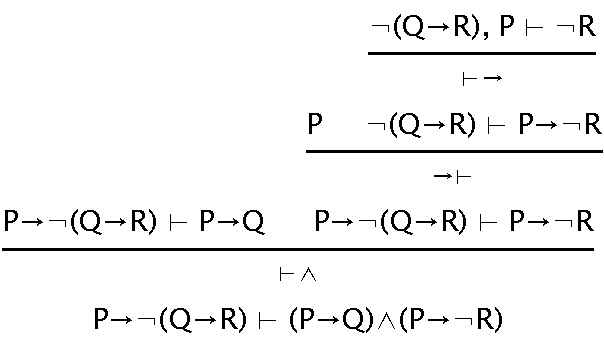
\includegraphics[scale=\picscale]{pics/firsttree}
\caption{a sequent tree, produced by backward reasoning}
\label{fig:firsttree}
\end{figure}

\subsection{A fake box-and-line display}

The proof attempt in \figref{firsttree} is doomed -- you can't prove $P$ from no hypotheses, so the middle tip won't close -- but it is a partial proof tree and it can be rendered in fake box-and-line style as in \figref{firsttreeboxed}, using a very simple recursive translation from the tree, starting at its root: 
\begin{enumerate}
%\item Start with an empty bag of hypotheses and consider the root of the tree. 
\item At a node which includes a hypothesis (left-side formula) which doesn't appear in its parent:
\begin{itemize}
\item  start a new box and write the new hypothesis (or hypotheses) as its first line, labelled ``assumption'';
\item write the conclusion (right-side formula of the node) on the final line; 
\item in between hypothesis and conclusion write the translations of all subtrees, working left to right;
\item label the final line with the name of the rule which generated the subtrees, the line number of the hypothesis formula which was reduced in the rule (if any), and the line numbers of the final line of each subtree representation -- or, if a box, the first and last line numbers of the box, separated by a hyphen;
\item if the node is a tip, don't label the final line -- instead precede it with a line of dots to show that it is an open conclusion.
\end{itemize}
\item At a node which doesn't introduce a new hypothesis, just do as above, but without the box and without the hypothesis line.
\end{enumerate}
 
\begin{figure}
\centering
\subfigure[simple rendering]{\centering
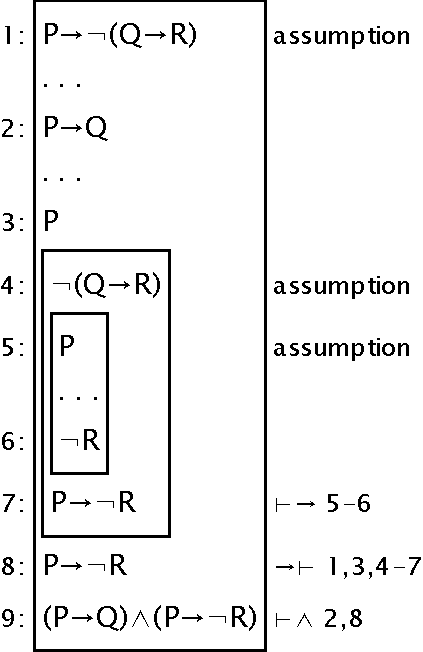
\includegraphics[scale=\picscale]{pics/firsttreeboxed}
\label{fig:firsttreeboxed}}
\qquad
\subfigure[box-and-line rules broken]{\centering
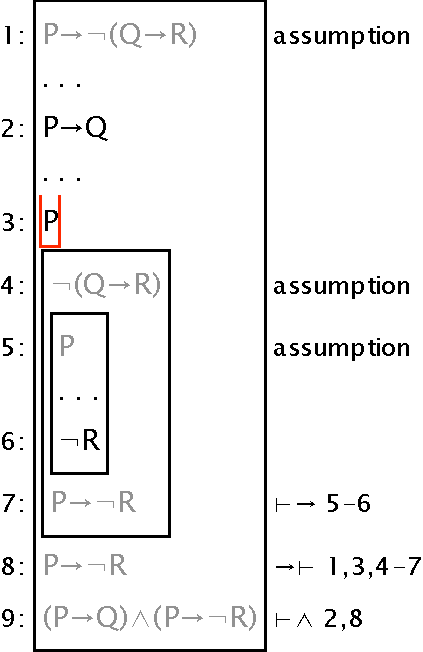
\includegraphics[scale=\picscale]{pics/firsttreeboxedgreyed}
\label{fig:firsttreeboxedgreyed}}
\caption{fake box-and-line rendering}
\label{fig:firsttreeboxedall}
\end{figure}

The root of the tree in \figref{firsttree}, for example, is represented by the box from lines 1 to 9 of \figref{firsttreeboxed}; it generated two subtrees by ⊢∧, whose conclusion lines are written on lines 2 and 8. Line 2 represents the left tip of the tree, which contains no new hypotheses. Lines 3 to 8 represent the right-hand side of the tree. The first step is  
→⊢, which reduced the hypothesis on line 1 and generated line 3 and the box from lines 4 to 7 \dots\ and so on.

\Figref{firsttreeboxed} looks like a box-and-line partial proof, but it isn't, and Jape will show you that it isn't if you click on one of the open conclusions on lines 2, 3 and 6. \Figref{firsttreeboxedgreyed} shows the result of clicking on line 3, which corresponds to the middle tip of the tree. $P->!(Q->R)$ on line 1 is greyed out, because it's a hypothesis which doesn't appear at that tip, and a greyed-out assumption can't be used. Line 2 isn't greyed out, but it's a conclusion line and can't be used as an assumption either. But in a real box-and-line proof you can appeal to any preceding line (which isn't enclosed in a box that you aren't also in) to make a step -- which means all assumption lines and even conclusion lines. It's clear that \figref{firsttreeboxedgreyed} is not a real box-and-line proof display.

Even fake box-and-line displays can be useful, though. It's not evident on this small example, but trees have some considerable disadvantages resulting from repetition of hypothesis and conclusion formulae. In \figref{firsttree}, for example, the hypothesis $P->!(Q->R)$ appears three times, while in \figref{firsttreeboxed} it appears once, on line 1. In \figref{firsttreeboxed} each conclusion appears only once, apart from $P->!R$ on lines 7 and 8. If there are a lot of large hypothesis formulae, the tree can get unmanageably wide on the page. The lack of repetition in the fake box-and-line display can be a great advantage, and its almost one-dimensional structure is much easier to traverse with the eye. Fake box-and-line displays are very popular with Jape users for just these reasons.

\subsection{Display style configuration}

The variable \textj{displaystyle} governs the tree/box display decision. Its values are \textj{tree} and \textj{box}, and for obvious historical reasons the default is \textj{tree}. The logic encoding can set the session default for new proof windows with an \textj{\textsc{initialise}}, and the user can alter it on a proof-by-proof basis. \textsc{scs.jt}, for example, includes commands in its \textsc{edit} menu to alter the setting:
\begin{japeish}
\begin{verbatim}
MENU "Edit"
    RADIOBUTTON displaystyle IS
        "Box display"   IS box
    AND "Tree display"  IS tree
    INITIALLY tree
    END
END
\end{verbatim}
\end{japeish}


\section{Hiding identity lines}

\Figref{secondtree} shows a completed proof in the calculus of \tabref{SCS}, and \figref{secondtreeboxed} its fake box-and-line rendering. In box view, every proof step of the tree is reproduced, and in particular all four uses of the hyp axiom are shown. But now these look like mere indirections: line 6, for example, is proved by ⊢∨(L) from line 5, which is proved by hyp from line 2, and apart from their labelling, lines 2 and 5 are identical. It simplifies the proof display to cut out the hyp-indirection, and to show \figref{secondtreeboxedidhidden}, in which all the hyp lines have been eliminated. Line 6 has become line 4, which points straight to line 2.

\begin{figure}
\centering
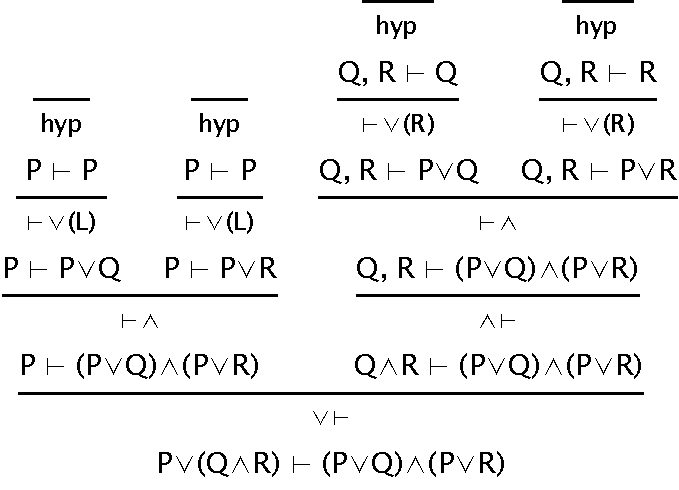
\includegraphics[scale=\picscale]{pics/secondtree}
\caption{A completed proof}
\label{fig:secondtree}
\end{figure}

\begin{figure}
\centering
\subfigure[simple rendering]{\centering
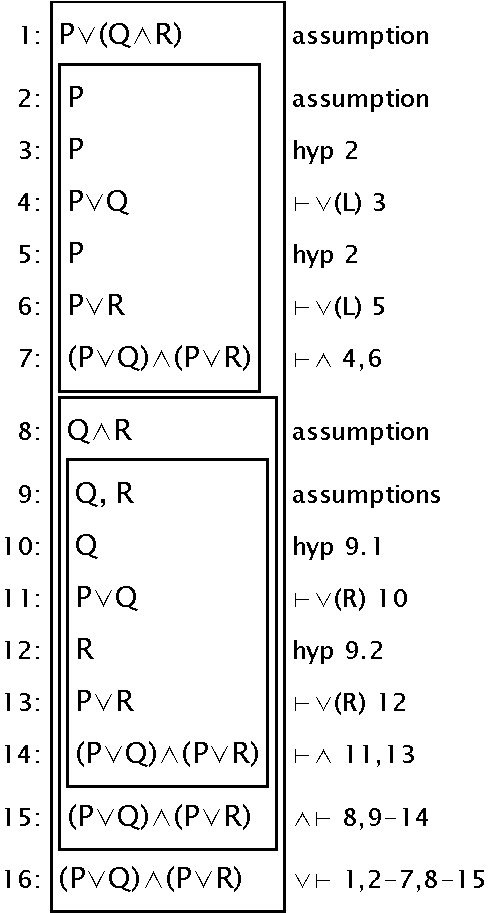
\includegraphics[scale=\picscale]{pics/secondtreeboxed}
\label{fig:secondtreeboxed}}
\qquad
\subfigure[identity lines hidden]{\centering
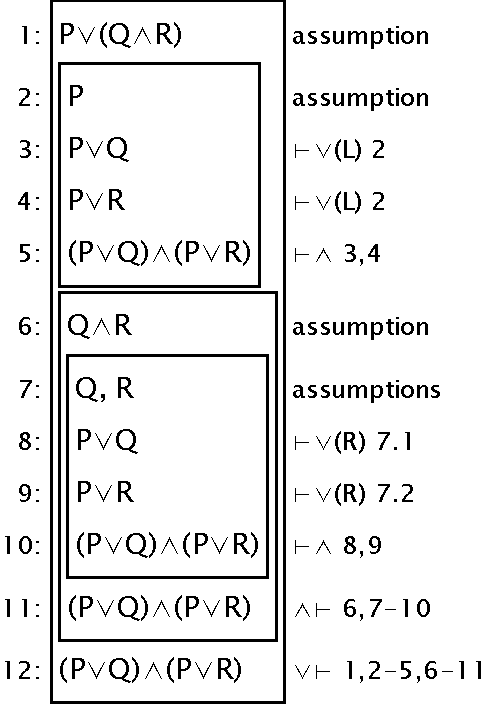
\includegraphics[scale=\picscale]{pics/secondtreeboxedidhidden}
\label{fig:secondtreeboxedidhidden}}
\caption{Fakery intensifies}
\label{fig:secondtreeboxedall}
\end{figure}

This is Jape's default rendering of fake box-and-line proofs. It isn't the same logic as the sequent logic, but it's possible from it to work out what the tree must be, behind the scenes, so it's not a dishonest rendering, and it's more compact so it's more useful.

\subsection{Identity line configuration}

If a rule is of the right kind -- a conclusion formula is eliminated by matching with an identical formula from the hypotheses, with no antecedent subproofs -- then it is a candidate for identity rule elimination. Declare the rule to be an identity rule -- \textsc{scs.jt}, for example includes a line
\begin{japeish}
STRUCTURERULE IDENTITY hyp
\end{japeish}
-- and set the variable \textj{hidehyp}\footnote{Apology for the historical name: clearly it ought to be \textj{hideidentitysteps} or something.} to \textj{true} (its default value).

\section{Forward steps from hypotheses}
\label{sec:firstforwardsteps}

\Tabref{I2L} shows the rules of a natural deduction calculus. It is possible to construct proofs by reasoning backward in this calculus, but it's awkward and it certainly isn't the way that provers want to use it. They prefer to construct proofs by reasoning forward from the premises as often as they can, and Jape can accommodate them. \Figref{forwardbox1}, for example, shows a forward step from $E$ and $E->F$ which deduces $F$. The next step would be to deduce $G$ from $F$ and $F->G$ to conclude $G$ and close the proof.

\word{actual}
\begin{table}
\centering
\caption{Natural deduction rules}
\label{tab:I2L}
\hstrut{5pt}\vstrut{5pt}\\
{\small
\begin{tabular}{|c|c|c|c|}
\hline
% ROW 0
\multicolumn{4}{|c|}{
\vstrut{15pt}
$\infer[\reason{hyp}]
       {\Gamma,A |- A}
       {}$}
\\
\hline
% ROW 1
\vstrut{25pt}
$\infer[\reason{→ elim}]
       {\Gamma  |- B}
       {\Gamma  |- A & \Gamma  |- A->B}$
& 
$\infer[\reason{∧ elim(L)}]
       {\Gamma  |- A}
       {\Gamma  |- A@B}$
& 
$\infer[\reason{∧ elim(R)}]
       {\Gamma  |- B}
       {\Gamma  |- A@B}$
& 
$\infer[\reason{¬ elim}]
       {\Gamma  |- \bot}
       {\Gamma  |- B & \Gamma |- !B}$
\\
\hline
% ROW 2
\multicolumn{2}{|c|}{
\vstrut{25pt}
$\infer[\reason{∨ elim}]
       {\Gamma |- C}
       {\Gamma |- A|B & \Gamma,A |- C & \Gamma,B |- C}$}
& 
\multicolumn{2}{|c|}{
$\infer[\reason{∀ elim}]
       {\Gamma  |- P(i) }
       {\Gamma  |- @*x.P(x)  & \Gamma |- \<actual> i}$} 
\\ 
\hline
% ROW 3
\multicolumn{4}{|c|}{
\vstrut{25pt}
$\infer[\reason{(\textsc{fresh} $i$, $i$ \textsc{notin} $|*x.P(x)$) ∃ elim}]
       {\Gamma  |- C}
       {\Gamma  |-|*x.P(x)  & \Gamma ,\<actual> i,P(i)  |- C}$
}
\\
\hline
% ROW 4
\vstrut{25pt}
$\infer[\reason{→ intro}]
       {\Gamma  |- A->B}
       {\Gamma,A |- B}$
& 
$\infer[\reason{→ intro}]
       {\Gamma  |- A@B}
       {\Gamma  |- A & \Gamma  |- B}$
& 
$\infer[\reason{∨ intro(L)}]
       {\Gamma  |- A|B}
       {\Gamma  |- A}$
& 
$\infer[\reason{∨ intro(R)}]
       {\Gamma  |- A|B}
       {\Gamma  |- B}$
\\
\hline
% ROW 5 
\vstrut{25pt}
$\infer[\reason{¬ intro}]
       {\Gamma  |- !A}
       {\Gamma,A |- \bot}$
&
$\infer[\reason{(\textsc{fresh} $i$) ∀ intro}]
       {\Gamma |- @*x.P(x) }
       {\Gamma,\<actual> i |- P(i) }$
& 
$\infer[\reason{∃ intro}]
       {\Gamma |-|*x.P(x) }
       {\Gamma  |- P(i)  & \<actual> i}$
&\\
\hline
% ROW 6
\vstrut{25pt}
$\infer[\reason{contra (classical)}]
       {\Gamma |- A}
       {\Gamma,!A |- \bot}$
&
$\infer[\reason{contra (constructive)}]
       {\Gamma |- A}
       {\Gamma |- \bot}$
&
$\infer[\reason{truth}]
       {\Gamma |- \top}
       {}$
&\\
\hline
\end{tabular}}
\end{table}

\begin{figure}
\centering
\subfigure[with cut hidden]{\centering
\fbox{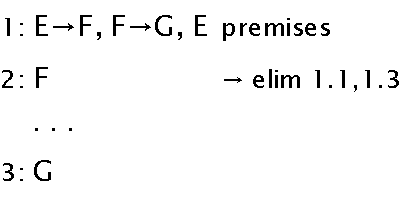
\includegraphics[scale=\picscale]{pics/forwardbox1}}
\label{fig:forwardbox1}}
\qquad
\subfigure[showing cut]{\centering
\fbox{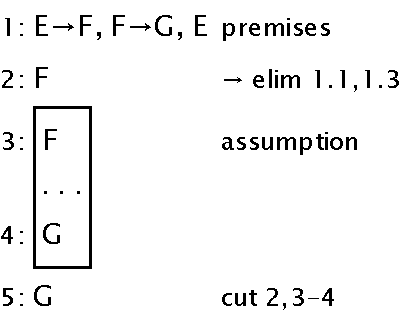
\includegraphics[scale=\picscale]{pics/forwardcut1}}
\label{fig:forwardcut1}}
\qquad
\subfigure[the tree]{\centering
\fbox{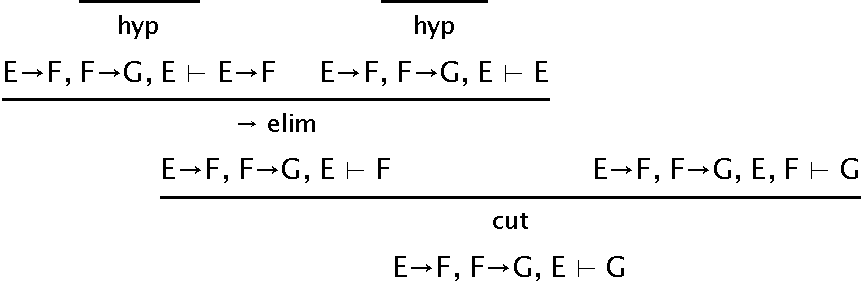
\includegraphics[scale=\picscale]{pics/forwardcut1tree}}
\label{fig:forwardcut1tree}}
\caption{Three views of a forward step}
\label{fig:forwardstep1}
\end{figure}

Figures \ref{fig:forwardcut1} and \ref{fig:forwardcut1tree} show what has really happened: a \textj{cut} step has introduced an additional hypothesis which can be used in the proof of $G$. The box display mechanism by default hides cut steps, conflating the left subtree's conclusion (line 2 of \figref{forwardcut1}) with the cut hypothesis (line 3) and the right subtree's conclusion (line 4) with the conclusion of the step (line 5), hiding entirely the box and the cut step justification (line 5). The result is a forward step that looks like a forward step, and can be used like a forward step.

\subsection{Configuration}
\label{sec:firstforwardstepsconfig}

This mechanism needs support from the prover. In \textj{ItL.jt} there is machinery to do the job. It's first necessary to distinguish between proof steps which can be applied forwards (elim steps, on the whole) and those which cannot (intro steps, on the whole) so, for example, the Rules menu contains the entries\footnote{The actual encoding uses -E and -I rather than elim and intro, but is otherwise as quoted here.}
\begin{japeish}
\begin{verbatim}
    ENTRY "∧ intro" 
    ...
    ENTRY "∧ elim(L)"  IS ForwardOrBackward ForwardCut 0 "∧ elim(L)"
    ENTRY "∧ elim(R)"  IS ForwardOrBackward ForwardCut 0 "∧ elim(R)"
\end{verbatim}
\end{japeish}
The first simply labels the ∧ intro rule, to be used backward at some conclusion (Jape will complain if it can't work out which conclusion to use), but the second introduces a tactic which first works out whether the rule is being used forward or backward. That tactic is
\begin{japeish}
\begin{verbatim}
TACTIC ForwardOrBackward (Forward, n, rule) IS 
  WHEN (LETHYP _P 
          (ALT (Forward n rule)
               (WHEN   
                  (LETARGSEL _Q 
                     (Fail (rule is not applicable to assumption ' _P ' 
                                    with argument ' _Q ')))
                    (Fail (rule is not applicable to assumption ' _P ')))))
       (ALT    
          (WITHSELECTIONS rule)
          (WHEN   
             (LETARGSEL _P
                (Fail (rule is not applicable with argument ' _P ')))
             (Fail (rule is not applicable))))
\end{verbatim}
\end{japeish}
Essentially, if the prover selects a hypothesis formula (\textj{LETHYP \_P}) then what you get is \textj{Forward n rule}, which in the case of the ∧ elim(L) entry turns out to be \textj{ForwardCut 0 "∧ elim(L)"}. If you don't select a hypothesis, you get \textj{WITHSELECTIONS rule}, which in the same case turns out to be \textj{WITHSELECTIONS "∧ elim(L)"}. If either of those tactics fails, then an error message is generated, which needn't detain us.

The \textj{ForwardCut} and \textj{ForwardUncut} tactics do the magic.
\begin{japeish}
\begin{verbatim}
TACTIC ForwardCut (n,rule)
    SEQ cut (ForwardUncut n rule)

TACTIC ForwardUncut (n,rule)
    (LETGOALPATH G (WITHARGSEL rule) 
                   (GOALPATH (SUBGOAL G n))  (WITHHYPSEL hyp) 
                   (GOALPATH G) NEXTGOAL)

\end{verbatim}
\end{japeish}
\textj{ForwardCut} inserts the cut, and then \textj{ForwardUncut} applies the rule. Then it goes to the $n$th subgoal of the rule and closes it with the selected hypothesis. The rest of the tactic has to do with navigating the tree when \textj{autoselect} is true and can safely be ignored.

\section{Why isn't it enough to hide cuts?}

The mechanism of \secref{firstforwardstepsconfig} looks good, and in \figref{forwardstep1} it is good, but in general it isn't good enough. There are two problems: 
\begin{itemize}
\item bifurcated proofs; 
\item and conclusion lines.
\end{itemize}

Consider, for example, \figref{bifurcated1}, produced by a single application of ∧ intro. In the box display it appears that a forward step of ∧ elim(L) will extract $F@G$, and then another couple of ∧ elims will extract $F$ for line 2 and $G$ for line 3. But from the tree it's clear that this is impossible: we have to apply a cut at one or other tip, and so we have to extract $F@G$ twice, once in each subproof. Provers are driven to plan to complete forward steps before backward steps, a burden they ought not to have to bear. Hiding \textj{cut}s alone doesn't do the job. 

\begin{figure}
\centering
\subfigure[in box form]{\centering
\fbox{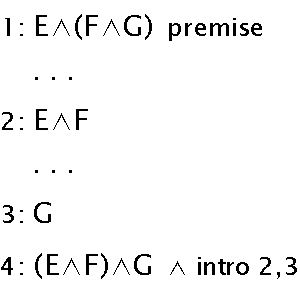
\includegraphics[scale=\picscale]{pics/bifurcatedbox1}}
\label{fig:bifurcatedbox1}}
\qquad
\subfigure[in tree form]{\centering
\fbox{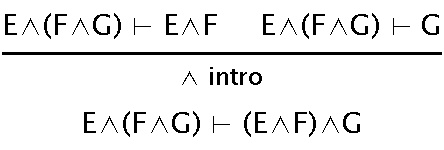
\includegraphics[scale=\picscale]{pics/bifurcatedtree1}}
\label{fig:bifurcatedtree1}}
\caption{Bifurcated proofs don't allow true forward steps}
\label{fig:bifurcated1}
\end{figure}

Just as bad is the fact that conclusion lines aren't usable as hypotheses in proving subsequent conclusions. It's made worse by the fact that lines introduced by forward steps look just like conclusion lines but can be used as hypotheses. In \figref{bifurcated2} a careful prover has made two forward steps first of all, introducing hypotheses $G$ and $F$ visible throughout the proof, as can be seen in the two cut steps in \figref{bifurcatedtree2}. Then the left tip ($G@F,F,G|-F@G$) has been closed with ∧ intro and a couple of hyps (hidden, of course, in the box display). It looks in the box display as if you could close the proof by hyp: line 6 can see line 4, and they are identical. But it's clear from the tree that you can't: there isn't a hypothesis $F@G$ anywhere in the tree.

\begin{figure}
\centering
\subfigure[in box form]{\centering
\fbox{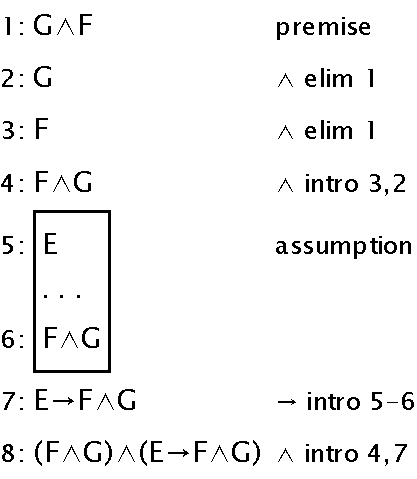
\includegraphics[scale=\picscale]{pics/bifurcatedbox2}}
\label{fig:bifurcatedbox2}}
\qquad
\subfigure[in tree form]{\centering
\fbox{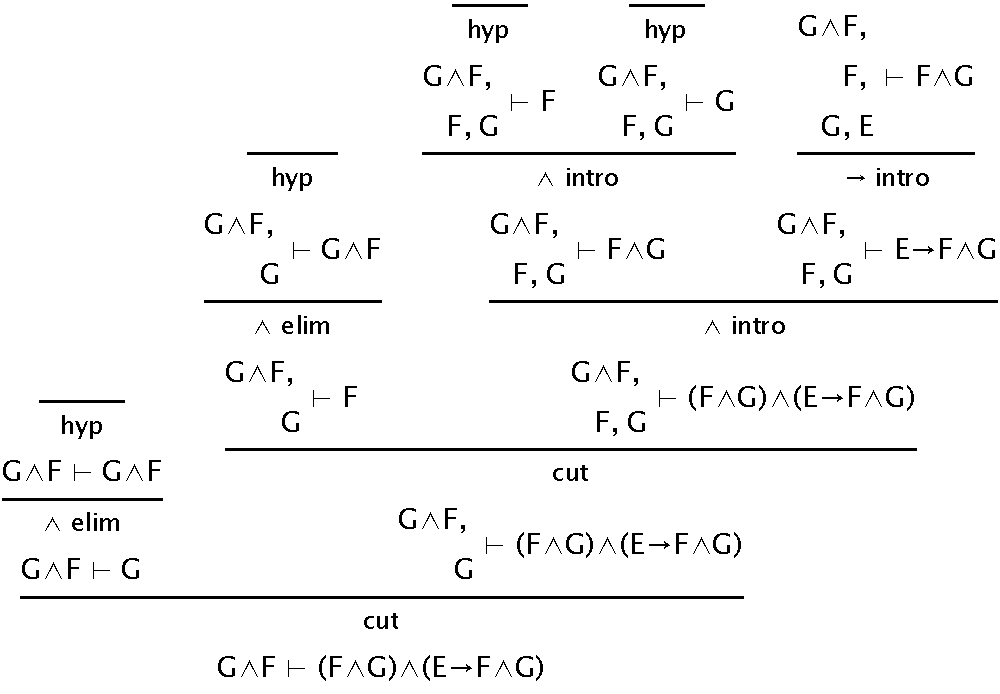
\includegraphics[scale=\picscale]{pics/bifurcatedtree2}}
\label{fig:bifurcatedtree2}}
\caption{Conclusion lines aren't hypotheses}
\label{fig:bifurcated2}
\end{figure}

We have to do something more drastic, and drastic it is.

\section{True forward steps with \tt{CUTIN}}

An alert prover can use the mechanism of \secref{firstforwardstepsconfig} most effectively by applying forward steps early, getting the cuts in low down in the tree, so that the extra hypothesis formulae they introduce are available to an entire tree. The same applies to forward steps from hypotheses inside a box: do them early, so that they are available to the entire box/subtree. But as you have seen, that isn't enough when a proof bifurcates. We need also to make conclusion lines into hypothesis lines. A single mechanism solves both problems: the built-in tactic \textj{CUTIN}, used for example in the \textj{I2L.jt} encoding.

Look first at what happens when a proof bifurcates, as in \figref{bifurcated3}. The box display looks exactly as it would if the proof had bifurcated, but you can see from the tree that it hasn't -- or at least the bifurcation is off to the side, and closed off by \textj{hyp}. The two conclusion lines have been cut in as hypotheses, and then the ∧ intro step simply appeals to those hypotheses. This time $F@G$ \emph{is} a hypothesis in the proof of $E->F@G$, and as soon as you apply → intro and introduce an open conclusion $F@G$ the earlier line is appealed to, as shown in \figref{bifurcated3a}.\footnote{Note that the \textj{hyp} step on line 4 can't be hidden: it isn't simply an indirection, it's an essential part of the box.}

\begin{figure}
\centering
\subfigure[as box]{\centering
\fbox{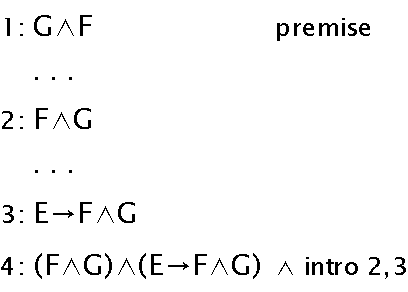
\includegraphics[scale=\picscale]{pics/bifurcatedbox3}}
\label{fig:bifurcatedbox3}}
\qquad
\subfigure[as tree]{\centering
\fbox{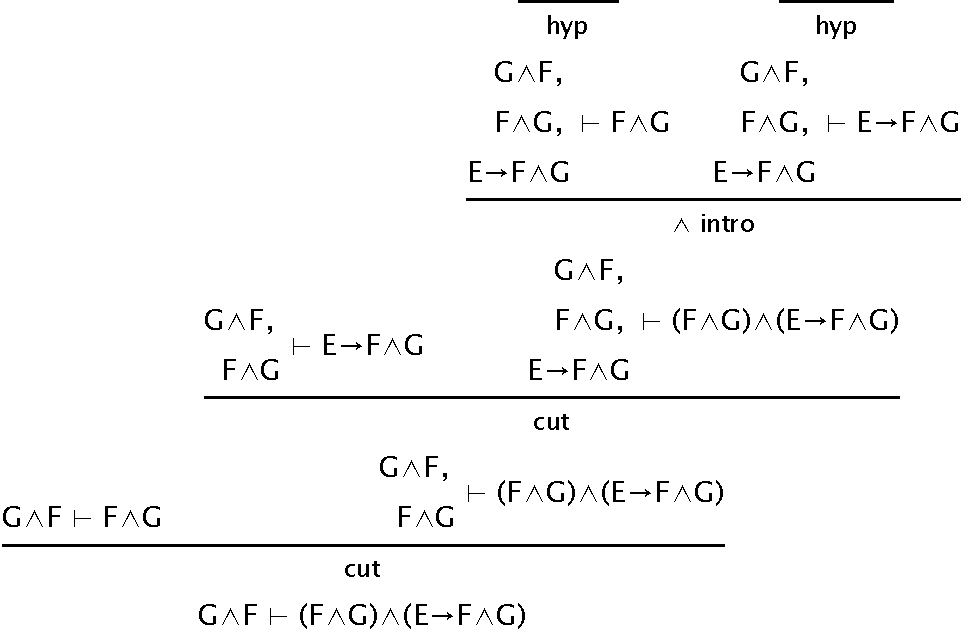
\includegraphics[scale=\picscale]{pics/bifurcatedtree3}}
\label{fig:bifurcatedtree3}}
\caption{Bifurcation conquered (preparation)}
\label{fig:bifurcated3}
\end{figure}

\begin{figure}
\centering
\subfigure[as box]{\centering
\fbox{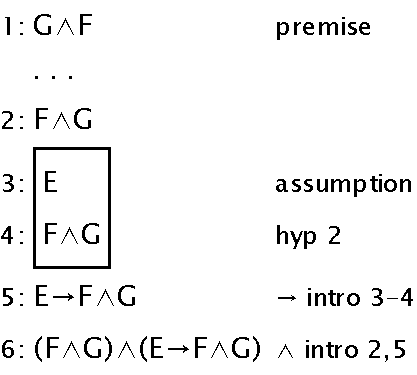
\includegraphics[scale=\picscale]{pics/bifurcatedbox3a}}
\label{fig:bifurcatedbox3a}}
\qquad
\subfigure[as tree]{\centering
\fbox{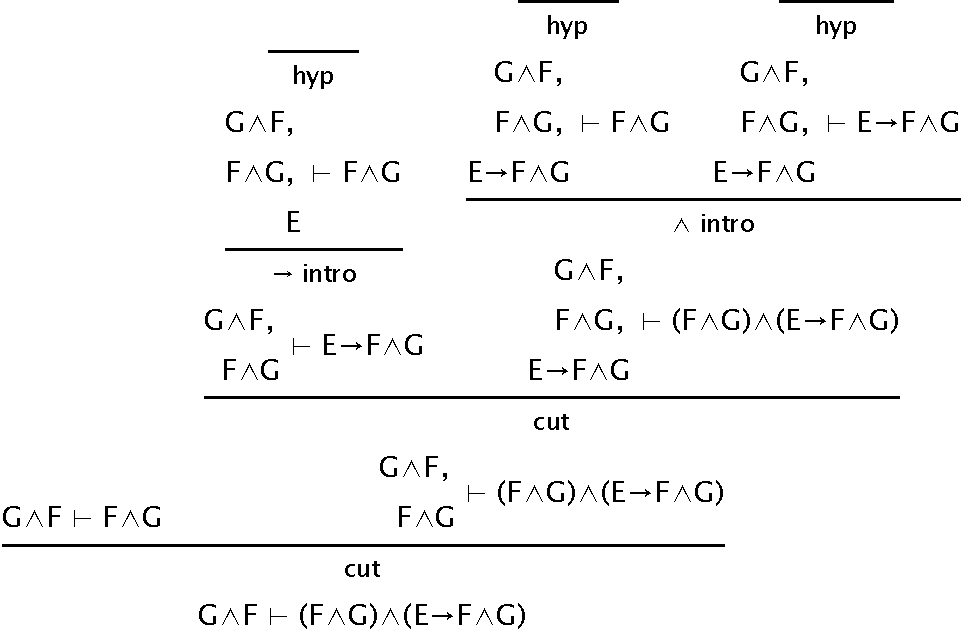
\includegraphics[scale=\picscale]{pics/bifurcatedtree3a}}
\label{fig:bifurcatedtree3a}}
\caption{Bifurcation conquered (use)}
\label{fig:bifurcated3a}
\end{figure}

In accommodating Jape to a much more aggressive use of \textj{cut}, I had to make some changes to the interpretation of formula selection. For some time Jape has shown conclusion-formula selections in box style with an upwards-opening red selection mark, as in \figref{firsttreeboxedgreyed}, for example, and hypothesis selections with a downwards-opening selection mark. But line 2 in \figref{bifurcatedbox3} stands for both an open conclusion at the left-hand subtree of a cut step -- that is, it has to be proved as a conclusion -- and a hypothesis in the entire right-hand subtree -- that is, it can be appealed to as an antecedent in proving subsequent lines. It's possible to select it in two ways, as illustrated in \figref{bothcutboxes}: for a conclusion selection click in the top half of the formula, for a hypothesis selection click in the bottom half, and in either case the closed end of the selection is dotted to show that it can be selected in the other direction.

\begin{figure}
\centering
\subfigure[as a conclusion]{\centering
\fbox{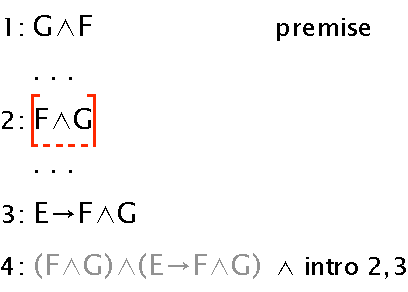
\includegraphics[scale=\picscale]{pics/upwardcutbox}}
\label{fig:upwardcutbox}}
\qquad
\subfigure[as a hypothesis]{\centering
\fbox{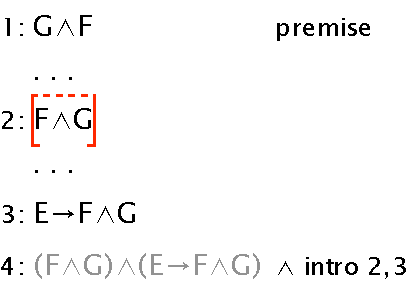
\includegraphics[scale=\picscale]{pics/downwardcutbox}}
\label{fig:downwardcutbox}}
\caption{Two ways of selecting a cut formula}
\label{fig:bothcutboxes}
\end{figure}

The other change is that it is now possible to select more than one hypothesis formula at a time, and that it is possible to select a hypothesis formula without selecting a conclusion, even if it is visible from several open conclusions (set \textj{seektipselection} to \textj{false}: Jape selects the lowest point in the tree at which that hypothesis occurs, which will almost always be a developed node, not a tip -- so only do it if you always interpret the hypothesis-only selection as mandating a forward step).

\subsection{What \tt{CUTIN} does}

Each selection (hypothesis and/or conclusion) corresponds to a unique point in the tree. \textj{CUTIN t} goes down the tree looking for the \emph{lowest} node which contains \emph{exactly} the same hypotheses as the selection, inserts a \textj{cut} node at that point with the previous tree as its right-hand side, augmenting each node in that tree to add the new cut hypothesis and adding \textj{NOTIN} provisos to make sure that it doesn't violate any \textj{FRESH} provisos, runs tactic \textj{t} on the left subtree of the \textj{cut}, and then returns to the original position. 

The effect is to add a new hypothesis to the tree, visible to every conclusion that could see the original hypotheses. There's some very nifty work which ensures that path expressions which are used to indicate a tree position still work even once the tree has been mangled with a \textj{cut}. There is a lot of checking to make sure you can do it soundly (\textj{autoAdditiveLeft} must be \textj{true}, which means the hypotheses are a bag and you don't worry about getting extra ones, and there must be exactly one cut rule).

It looks like extreme violence to the tree, which it is, and you might wonder as I did whether it would be easier if I used a box-and-line structure from the first. When I thought hard about it I decided that it would be about as difficult to make a forward step in such a case as it is with the tree, and there is a lot of investment in the tree in Jape as it actually exists. I can't imagine going beyond this hack, though ...

\subsection{Configuration: forward steps with \tt{CUTIN}}

The \textj{I2L.jt} encoding is complicated by error reporting, but in principle it uses the same technique as \secref{firstforwardstepsconfig}, but using \textj{CUTIN} rather than \textj{cut} (see \textj{I2L\_menus.j}). It works better than the earlier technique, because every line that can see the hypothesis you are reducing gets to see the result of the step too. It is possible to do silly things, but if you start with a situation that obeys the box-and-line rules, then the situation after the forward step also obeys the rules.

\subsection{Configuration: backward steps with \tt{CUTIN}}

Every time you produce a new conclusion with a backward step, whether it's a bifurcating step or not, you want to make it visible to open conclusion lines below it in the proof -- only the ones that can validly see it, of course. There are a couple of tactics in \textj{forwardstep.j} that do the job using \textj{CUTIN}.

First, the badly-named \textj{trueforward} (which is a macro rather than a tactic, and I've forgotten why):
\begin{japeish}
\begin{verbatim}
MACRO trueforward(tac) IS
    LETGOAL _A 
        (CUTIN (LETGOAL _B (UNIFY _A _B) tac)) 
        (ANY (MATCH hyp))
\end{verbatim}
\end{japeish}
\textj{trueforward t} records the conclusion of the node it's applied to, which has to be a tip. Then it \textj{CUTIN}s a new hypothesis, which it makes the same as the original conclusion, runs tactic \textj{t}, and when that finishes, goes back home and closes the original node by \textj{hyp}.\footnote{I ought to make the identity rule it uses a parameter.} The effect is that \textj{t} is run much lower down the tree, and if each conclusion is treated with \textj{fstep}...

The \textj{fstep} tactic just makes a hypothesis out of the conclusion of the node it's applied to. In effect, that introduces a conclusion which is produced in the left subtree of a cut as a hypothesis in the main spine of the tree. 
\begin{japeish}
\begin{verbatim}
TACTIC fstep IS
    ALT (ANY (MATCH hyp)) (trueforward SKIP)
\end{verbatim}
\end{japeish}
-- either find a hypothesis which matches by identity, or use \textj{trueforward} to insert it as a new hypothesis. Very useful, used all over the place in \textj{I2L.jt}, and even more subtly in \textj{hoare.jt}.

\section{Summary}

If your encoding applies \textj{CUTIN (ForwardCut ...)} to forward steps which don't introduce a box (in natural deduction everything except ∨ elim and ∃ elim) and \textj{fstep} or \textj{trueforward} every time it introduces a conclusion, you get proof displays which obey the box-and-line rules. 

A prover can mess it up by applying rules directly with File:Text Command. If you want to fix that, you probably have to make a version of Jape which uses a box-and-line structure rather than a tree in the background. Feel free!

\bibliographystyle{plain}
\bibliography{bornat} 

\end{document}